% Shared typography for the Curious Signals topic papers.
\documentclass[journal]{IEEEtran}
\usepackage[T1]{fontenc}
\usepackage[utf8]{inputenc}
\usepackage{lmodern}
\usepackage{amsmath,amssymb,bm}
\usepackage{graphicx,booktabs,array}
\usepackage{siunitx}
\usepackage{tikz}
\usetikzlibrary{arrows.meta,positioning,calc,decorations.pathmorphing}
\usepackage{pgfplots}
\usepgfplotslibrary{groupplots}
\pgfplotsset{compat=1.18}
\usepackage{cite,microtype}
\usepackage[hidelinks]{hyperref}
\usepackage{xurl}
\definecolor{csblue}{HTML}{245B78}
\definecolor{csred}{HTML}{B65338}
\definecolor{csteal}{HTML}{278078}
\definecolor{csgold}{HTML}{967135}
\definecolor{csgray}{HTML}{62676C}
\renewcommand{\unit}[1]{\ensuremath{\,\mathrm{#1}}}
\newcommand{\code}[1]{\texttt{#1}}
\newcolumntype{P}[1]{>{\raggedright\arraybackslash}p{#1}}
\newcommand{\sourcecommit}{0a5cf6f}
\newcommand{\editiondate}{October 27, 2026}
\newcommand{\paperauthors}{Sebastian J. Spicker, Alexander K\"upper}
\pgfplotsset{every axis/.append style={
  width=0.98\columnwidth,height=4.8cm,
  label style={font=\footnotesize},tick label style={font=\scriptsize},
  legend style={font=\footnotesize,draw=none,fill=white},
  axis line style={black!65},tick style={black!65},
  grid style={black!12},major grid style={black!12},
  scaled ticks=false,
  unbounded coords=jump,
  axis on top,
  axis background/.style={fill=white}
}}
\tikzset{>=Latex,every node/.style={font=\footnotesize}}
\setlength{\emergencystretch}{1em}
\newcommand{\dataprovenance}{Data provenance: the datasets analysed in this
  paper are deterministic example data, generated for the October 2026 edition from fixed
  seeds by the scripts in \texttt{example-data/}. They are modelled on the named
  sensors' units, sampling, resolution, noise and limits; they are not
  recordings from the original work. The date above is the author's
  approximate dating of that work, not of these data.}
\newcommand{\makepapertitle}{%
  \hypersetup{pdftitle={\papertitle},pdfauthor={\paperauthors},
    pdfsubject={Measurements and laboratory models; \paperperiod; collected edition \editiondate},
    pdfkeywords={physics education, instrumentation, calibration, uncertainty, phyphox}}%
  \title{\fontsize{21}{25}\selectfont\papertitle}%
  \author{Sebastian~J.~Spicker, Alexander~K\"upper\\[0.5ex]
    {\normalsize Institute of Physics Education\\University of Cologne, Germany
      \quad\textperiodcentered\quad\paperperiod}\thanks{\dataprovenance}}%
  \markboth{Curious Signals --- Measurements and Laboratory Models}%
    {Spicker and K\"upper: \papershorttitle}%
  \maketitle
}

\usepackage{flafter}
\newcommand{\papertitle}{Inverse-Square Photometry: Distance, Timing and Averaging}
\newcommand{\papershorttitle}{Inverse-Square Photometry}
\newcommand{\paperperiod}{March 2020}
\newcommand{\experimentfile}{experiments/drafts/illuminance-distance.phyphox}
\begin{document}
\makepapertitle
\begin{abstract}
An inverse-square photometry experiment tests a distance dependence only after light and position have been associated with the same optical state. Two example investigations compare electronically tracked position with paired ruler observations. Fifteen stationary electronic windows give a power exponent of 2.0012. Twelve ruler snapshots give 1.9861; replacing each snapshot with a two-second interior mean gives 1.9880 while reducing the scatter of the distance-normalized signal from 1.82 to 0.58 count\,m$^2$. A one-millimetre change of distance origin shifts either mean-based exponent by approximately 0.005--0.006. Together the examples distinguish improvements in temporal averaging from knowledge of source geometry, background and the absolute photometric scale.
\end{abstract}
\begin{IEEEkeywords}
Inverse-square law, photometry, distance calibration, paired observations, averaging, finite sources.
\end{IEEEkeywords}

\section{A common distance model}
A detector moved away from a compact lamp receives less light, but the appearance of a decaying curve does not identify its cause. Source dimensions, detector orientation, background and the definition of distance all enter the comparison. Electronic tracking and a ruler can supply the same independent variable; their different acquisition paths chiefly change how a light reading is assigned to a position.

For a point source observed along a fixed direction, the illuminance on a perpendicular detector obeys
\begin{equation}
 E_v(r)-B=\frac{I_v}{r^2},
 \label{eq:illuminance-distance-law}
\end{equation}
where $I_v$ is luminous intensity and $B$ a lamp-independent background. The distance runs from a defined source centre to the detector reference plane. Photometric calibration practice controls these reference locations and the distance range over which finite-source departures are negligible\cite{zong2018}. An extended source can produce a different dependence at short distances\cite{campione2024}. Background isolation is likewise part of the physical test; Vera and colleagues explicitly addressed this problem in an inverse-square experiment under daylight conditions\cite{vera2014}.

A relative detector supports the corresponding shape test without an absolute illuminance calibration. With fixed source spectrum, geometry and linear response, its background-corrected signal $Q=C-B$ can be fitted as
\begin{equation}
 Q=A(r/1\unit{m})^{-n}.
 \label{eq:illuminance-distance-power}
\end{equation}
The target exponent is $n=2$. The amplitude $A$ retains the detector's units: lux for the SensorTag example and counts for the Nano example. Thus the two investigations test the same geometrical dependence while carrying different information about the signal scale. Their independent runs compare the geometrical dependence on each detector's own signal scale.

\section{Assigning light to a stationary position}
Figure~\ref{fig:illuminance-distance-apparatus} shows a common rail arrangement. Fix the source direction, detector aperture and carriage orientation. A ruler establishes the source-to-aperture distance; an attached mouse can subsequently track changes without replacing that length calibration. Stop at each position before selecting a light observation.

\begin{figure}[t]
\centering
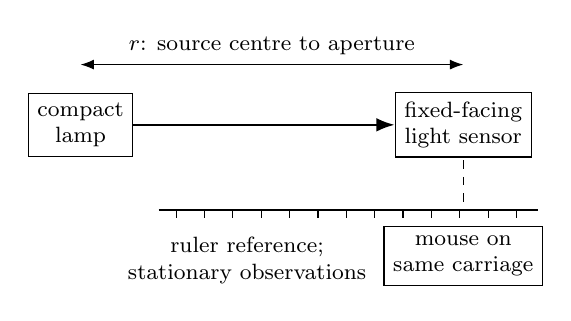
\begin{tikzpicture}[x=0.9cm,y=0.9cm]
 \node[draw,align=center] (s) at (.65,1.2) {compact\\lamp};
 \node[draw,align=center] (d) at (6.05,1.2) {fixed-facing\\light sensor};
 \draw[->,thick] (s.east)--(d.west);
 \draw[thick] (1.75,0)--(7.1,0);
 \foreach \x in {2,2.4,...,6.8}{\draw (\x,0)--(\x,-.12);}
 \draw[dashed] (6.05,.7)--(6.05,0);
 \node[draw,align=center] at (6.05,-.65) {mouse on\\same carriage};
 \draw[<->] (.65,2.05)--(6.05,2.05);
 \node[above] at (3.35,2.05) {$r$: source centre to aperture};
 \node[below,align=center] at (3.0,-.25) {ruler reference;\\stationary observations};
\end{tikzpicture}
\caption{One rail supports two position methods. Ruler observations supply distance directly; electronic tracking uses a separately calibrated count scale and origin. Both retain the detector's orientation and optical reference plane.}
\label{fig:illuminance-distance-apparatus}
\end{figure}

For electronic tracking, signed mouse increments accumulate into coordinates $x$ and $y$. On a straight rail restricted to one side of the origin,
\begin{equation}
 d=\sqrt{x^2+y^2},\qquad r=r_0+kd.
 \label{eq:illuminance-distance-rail}
\end{equation}
The example uses $r_0=0.15\unit{m}$, $k=2.0\times10^{-4}\unit{m/count}$ and an initial position of 250 counts, corresponding to $0.20\unit{m}$. The initial position is part of the calibration, rather than an additional distance inferred from the light signal. The norm is displacement from the reset origin, not accumulated travel length; unrestricted curved motion or crossing the origin would require a signed rail coordinate.

Light and mouse reports have separate receive times. For each light time $t_i$, select the mouse report with the largest timestamp not exceeding $t_i$. This previous-position rule retains elapsed time and avoids pairing equal row numbers from unequal-rate streams. Its physical justification is strongest during a stationary interval. During motion, an old position report and unequal delivery delays can change the apparent light--position relation. Missing notifications leave time gaps rather than a compressed time axis.

The electronic example has light readings spaced by $0.8\unit{s}$. For station $j=0,\ldots,14$, use the half-open receive-time window $[4j+1,4j+3.5)\unit{s}$. Each contains three readings inside a stationary state. Previous-position association reproduces the example distances to numerical rounding. The OPT3001 conversion from its result word is consistent with the illuminance indication\cite{opt3001}; this checks numerical scaling separately from the mounted detector's responsivity. Subtract the adopted $2\unit{lx}$ background before fitting.

The ruler investigation instead supplies twelve paired observations: positions 0.20, 0.30, 0.40, 0.50, 0.60 and $0.70\unit{m}$ outward, followed by the same positions in reverse order. Each observation identifies a light snapshot by its device time, receive time and captured count. Matching these quantities to the continuous light sequence establishes the association without interpolating ruler positions. The APDS-9960 clear response remains a relative count\cite{apds9960}.

Subtract a 10-count background. A second estimator averages the continuous light over $[5j+1.5,5j+3.5)\unit{s}$ on the device clock, for $j=0,\ldots,11$. These two-second interior windows contain approximately forty readings and exclude state changes. Snapshot and interval mean then describe the same ruler position using different temporal support. Averaging the light readings cannot retroactively improve the length observation.

\section{Shape, averaging and return travel}
Fit $\ln Q$ against $\ln(r/1\unit{m})$ by unweighted least squares. Equal weights in logarithmic signal emphasize fractional deviations rather than the much larger absolute signals near the lamp. All corrected signals in these reductions are positive. Table~\ref{tab:illuminance-distance-fits} reports the three estimators; Fig.~\ref{fig:illuminance-distance-results} displays the electronic fit and the ruler comparison.

\begin{table}[t]
\caption{Power-law fits to stationary-window means and ruler snapshots. Log-residual SD summarizes station-to-station scatter in $\ln Q$.}
\label{tab:illuminance-distance-fits}
\centering\small
\begin{tabular}{@{}lrrr@{}}
\toprule
Position/light estimator & States & $n$ & Log SD\\
\midrule
Electronic / stationary mean & 15 & 2.0012 & 0.00766\\
Ruler / snapshot & 12 & 1.9861 & 0.01743\\
Ruler / two-second mean & 12 & 1.9880 & 0.00195\\
\bottomrule
\end{tabular}
\end{table}

\begin{figure}[t]
\centering\begin{tikzpicture}
\begin{groupplot}[group style={group size=1 by 2,vertical sep=1.2cm},
width=0.98\columnwidth,height=3.7cm,grid=major,enlarge x limits=0.03,
legend style={font=\scriptsize,at={(0.5,1.03)},anchor=south,legend columns=2,draw=none,fill=none},
title style={font=\scriptsize,at={(0.02,0.98)},anchor=north west,fill=white,inner sep=2pt},
label style={font=\footnotesize},tick label style={font=\scriptsize}]
\nextgroupplot[ylabel={$Q$ (lx)},xmin=0.18,xmax=0.83,ymin=0,ymax=3000,title={(a) Electronically paired states}]
\addplot[csblue,only marks,mark=*,mark size=1.4pt] table[col sep=comma,x=c0,y=c1] {data/drafts/optics-distance-observations.csv};
\addlegendentry{Station means}
\addplot[csred,dashed,thick] table[col sep=comma,x=c0,y=c1] {data/drafts/optics-distance-fit.csv};
\addlegendentry{Power-law fit}
\nextgroupplot[ylabel={$Qr^2$ (count m$^2$)},xlabel={Source-to-aperture distance (m)},xmin=0.18,xmax=0.83,ymin=99,ymax=107,title={(b) Ruler: snapshot versus mean}]
\addplot[csblue,only marks,mark=*,mark size=1.4pt] table[col sep=comma,x=c0,y=c2] {data/drafts/optics-manual-observations.csv};
\addlegendentry{Snapshot}
\addplot[csteal,only marks,mark=triangle*,mark size=1.7pt] table[col sep=comma,x=c0,y=c4] {data/drafts/optics-manual-observations.csv};
\addlegendentry{Two-second mean}
\end{groupplot}
\end{tikzpicture}

\caption{Upper: stationary-window light means and power-law fit for electronic positions. Lower: ruler snapshots and two-second means expressed as $Qr^2$, showing reduced scatter after averaging. The independent sequences retain lux and count scales.}
\label{fig:illuminance-distance-results}
\end{figure}

The electronic fit gives $A=103.18\unit{lx}$ and $n=2.0012$. Its mean $Qr^2$ is $103.28\unit{lx\,m^2}$ with between-window sample SD $0.76\unit{lx\,m^2}$. A stable responsivity error would rescale every product while leaving the exponent largely unchanged. The exponent tests the distance dependence, while the absolute intensity $I_v$ also depends on detector responsivity.

For the ruler observations, the mean product changes only from 102.48 to $102.81\unit{count\,m^2}$ when snapshots are replaced by interval means. Its sample SD falls from 1.82 to $0.58\unit{count\,m^2}$, while the exponent changes by less than 0.002. This reduction of scatter identifies a contribution from the instantaneous light reading. It does not remove the modest increase of the averaged product with distance.

Return travel also retains information that a single fitted line can conceal. At $0.20\unit{m}$, the averaged outward and return products are 102.24 and $101.90\unit{count\,m^2}$; at $0.70\unit{m}$ they are 103.62 and $103.37\unit{count\,m^2}$. The small within-position differences coexist with a larger change across the rail. Repeated positioning and a distance-dependent bias are consequently different questions, even when both enter the scatter of a global fit.

\section{Distance origin and the interpretation of residuals}
An origin error changes every station coherently. Shifting all electronic distances by $-1\unit{mm}$ or $+1\unit{mm}$ gives exponents 1.9962 and 2.0062. The same perturbations applied to the ruler interval means give 1.9824 and 1.9936. These are sensitivity calculations under changed geometrical assumptions, not confidence limits. Their size is comparable to the deviations that might otherwise be assigned to the inverse-square law.

Deleting one electronic stationary window at a time gives exponents from 1.9966 to 2.0032. That diagnostic concerns which stations constrain the fit; it cannot determine a shared origin error. Similarly, more light samples at one station constrain that optical state without creating new independent positions. For the ruler example, each position assignment remains common to the snapshot and approximately forty readings in its mean.

Background error has another recognizable dependence. A residual additive offset $\Delta B$ contributes $\Delta B r^2$ to the inverse-square product, becoming relatively more important at distant stations. A source-centre error instead changes the distance argument and can introduce curvature. Finite source extent is most consequential nearby. The remaining trend should therefore be assessed against these physically distinct alternatives before adding detector-response parameters.

For an ideal product, small independent errors contribute relative terms $u(Q)/Q$ and $2u(r)/r$. Here background, origin and count scale are shared across stations, so their joint covariance belongs in any uncertainty assigned to source intensity or exponent. Lamp ripple and repeated integration can also correlate adjacent readings. The applicability of a $1/\sqrt N$ uncertainty law depends on those correlations and the independence of repeated replacements.

Both examples support an inverse-square description over their selected ranges. Their complementary contribution is methodological: electronic timing makes light--position association explicit, while snapshots and interval means separate instantaneous light scatter from geometrical knowledge. Absolute photometry additionally requires a calibrated optical response, a defined aperture and a traceable length scale. Those requirements remain even when the normalized product looks nearly constant.

\bibliographystyle{IEEEtran}
\bibliography{references}
\end{document}
